\documentclass{article}
\usepackage{enumitem}
\usepackage{indentfirst}
\usepackage{amsfonts}
\usepackage{hyperref}           % Use links
\usepackage{graphicx}           % Coloque figuras
\usepackage{epstopdf}
\usepackage{float}              % [...] no lugar adequado!
\usepackage[T1]{fontenc}        % Encoding para português 
\usepackage{lmodern}            % Conserta a fonte para PT
\usepackage[portuguese]{babel}  % Português
\usepackage{hyphenat}           % Use hifens corretamente

\graphicspath{{./img/}}

\hyphenation{mate-mática recu-perar}

\setlist{  
    listparindent=\parindent,
    parsep=0pt,
}

\def\code#1{\texttt{#1}}

\author{\textbf{Igor Lacerda Faria da Silva\( ^1 \)} }

\title{\textbf{Trabalho Prático 2}

\textbf{Ordenação em Memória Externa}}

\date{%
    \( ^1 \)Departamento de Ciência da Computação - Universidade Federal de Minas Gerais (UFMG) - Belo Horizonte - MG - Brasil \\ [2ex]
    \href{mailto:igorlfs@ufmg.br}{\nolinkurl{igorlfs@ufmg.br}}
}

\begin{document}

\maketitle

\section{Introdução}

O problema proposto foi implementar um \textit{classificador de URLs} (com base em uma quantidade de visitas e ordem alfabética como desempate), que usa tanto a memória principal como a memória secundária. Um \textit{classificador de URLs} com essa propriedade pode ser útil em situações em que a memória principal do computador é insuficiente. O arquivo de entrada é lido e ordenado em \textit{rodadas}, que posteriormente são intercaladas para formar um arquivo final contendo todas as URLs em ordem.

Esta documentação tem como proposta explicar como se deu essa implementação, desde questões mais ligadas ao funcionamento do programa (Seção 2) como análises de complexidade (Seção 3) e experimentais (Seção 4). Ao final do texto, encontra-se uma conclusão (contendo o aprendizado pessoal do autor com o trabalho), bibliografias e, por último, as instruções para compilação e execução.

\section{Método}

O programa foi desenvolvido em C++ e compilado utilizando o g++, do GCC. A máquina que foi usada durante o desenvolvimento conta com 12Gi de memória RAM, e processador AMD Ryzen 7 5700U, e roda o sistema operacional GNU/Linux (versão do kernel: 5.15.13).

A formatação do código fonte (\textbf{incluindo a indentação}): \textbf{foi feita usando a ferramenta clang-format}. Foi usado um arquivo customizado para isso, que se encontra na raiz do projeto, com o nome de \textit{.clang-format}. É um arquivo bem curto, baseado em preferências pessoais do autor, mas que \textbf{garante a consistência da formatação do projeto}.


\subsection{Organização do código}

O projeto atende à especificação no que diz respeito à organização do código de forma geral (implementações em \code{./src}, etc). Em particular, a única divergência é que os \emph{headers} usam a extensão \code{.hpp} e não \code{.h}. Ao todo são 5 arquivos de código em si\footnote{Excluindo subprogramas usados nas análises.}: um arquivo que executa o programa principal, uma definição e implementação de um Heap e por fim uma definição e implementação de uma classe \code{Fita}. Adicionalmente, é definido uma classe \code{Page} no mesmo arquivo da \code{Fita} para simplificar a implementação de alguns requisitos.

A estrutura \code{Page} a princípio tinha o propósito de substituir o uso de um \code{std::pair}, que (provavelmente) é proibido nos TPs, mas acabou ajudando também na hora de definir uma ordem customizada, mantendo na frente quem vem antes na ordem alfabética. Além disso, ela quebrou um galho na hora de intercalar, evitando buscas desncessárias com a adição do membro inteiro \textit{round}. A classe \code{Fita} gerencia a operação inicial (de leitura, ordenação e escrita), enquanto a classe \code{Heap} é responsável pela de intercalação.

Com respeito às boas práticas, foi usado \textit{camelCase} nos nomes das variáveis e métodos (fora nomes tradicionais). O nome das classes começa com letra maiúscula. Como houve certa confusão na especificação dos parâmetros, destaco aqui que meu programa funciona com apenas 3, nessa ordem: nome do arquivo de entrada, nome do arquivo de saída e número de ``entidades'' por rodada.

\subsection{Estruturas de Dados, TADs e métodos}

A estrutura de dados canônica deste TP é o Heap, mas adicionalmente há a classe \code{Fita} (fora a \code{Page} cujo uso já foi comentado). Na \code{Fita}, de fato, também não há nada ``de novo'' em termos de estrutura, mas sim \textit{implementação:} uso do QuickSort. A Fita não possui membros, mas faz uma alocação dinâmica, enquanto o Heap possui um ponteiro de \code{Page}.

\subsubsection{Fita}

O método principal da \code{Fita} é o \code{sortFitas()}, que lê as linhas dos arquivos (\code{read()}), os ordena em memória usando o QuickSort e escreve os arquivos de saída ordenados (\code{write()}). Aqui vale um agradecimento à Raquel Prates, pelas aulas e por disponilizar o código que serviu de base para a implementação da ordenação.

No QuickSort, é escolhido um pivô, que é usado como base para que sejam realizadas trocas sucessivas entre elementos que estão antes e depois dele. Nos caminhamentos, para a direita, se o elemento for maior que o pivô e para a esquerda, se for menor que o pivô, os elementos são trocados, continuando até que os caminhos se cruzem. Assim, o pivô vai terminar na posição correta. São feitas chamadas recursivas para completar o processo.

\subsubsection{Heap}

Um \textit{heap} funciona como uma árvore binária, mas é organizado como um arranjo, o que faz com que ele ocupe menos espaço. Para realizar isso, o \textit{heap} conta com a seguinte propriedade: dado um de seus elementos \( i \) até a metade, para sua ``chave'' \( c[i] \) vale que \( c[i] \geq c[2i] \land c[i] \geq c[2i+1] \). Na classe \code{Heap} são implementadas algumas operações deste tipo: construição (\code{build()}), inserção (\code{push()}), remoção (\code{pop()}) e também operações relacionadas à aplicação, como leitura (\code{read()}) e intercalação. Alguns procedimentos também foram inspirados nas aulas da professora Raquel Prates.

Na implementação, na primeira ``fase'' do Heap, os arquivos com as rodadas são abertos, uma entrada de cada um é lida e constrói-se o \code{Heap} com uma \code{Page} de cada rodada. Isso é interessante pois os arquivos não são fechados nessa etapa, para que a inserção continue após a primeira leitura. Na construção, é chamado o método \code{remake()}, que arruma a condição do \textit{heap} mencionada anteriormente. Na segunda ``fase'' (intercalação), são realizadas as remoções e (possivelmente) inserções, que também chamam internamente o \code{remake()}. Como uma inserção somente ocorre após uma remoção, há certa facilidade em não ser necessário se preocupar com o redimensionamento do arranjo.

\section{Análise de Complexidade}

A seguir, são analisadas as complexidades de tempo e de espaço dos principais métodos do classificador. Presume-se que algumas funções padrão de C++ são \( \Theta(1) \). Alguns métodos simples somente serão comentados brevemente aqui, na abertura da seção.

Tanto a leitura como a escrita da fita são \( \Theta(1) \) no espaço (porque não alocam memória a depender dos parâmetros) e \( \Theta(n) \) no tempo, pois percorrem todo o arranjo, sequencialmente. A leitura do heap segue um racioncínio semelhante. Na construção do \code{Heap}, é feita uma alocação de  \( n + 1 \) posições na memória, ou seja, ele é \( \Theta(n) \) no espaço e no tempo é \( \Theta(1) \). O método para escolha dos pivôs é constante. A função \code{sortFitas()}, excluindo o espaço do \code{quickSort()}, também faz a alocação de \( n \) elementos, nesse sentido sendo \( \Theta(n) \) no espaço. Como seu laço é composto de 3 operações, duas \( \Theta(n) \) e uma \( \Theta(n \log n) \) (\( n \) sendo o número de páginas por fita), o laço é \( \Theta(n \log n) \) em tempo, e supondo \( K \) linhas a serem lidas no arquivo, o laço é executado \( \lceil K/n \rceil \) vezes, portanto a função é \( \Theta(K\log n) \) no tempo.

\begin{itemize}

	\item \code{quickSort()}

	      \textbf{Tempo:} O método de partição (\code{partition()}) sempre caminha o equivalente ao tamanho do arranjo, e com as chamadas recursivas ao \code{sort()}, a análise precisa ser divida em casos. No melhor caso, cada partição divide o conjunto em duas partes iguais, o que resulta numa recorrência que pode ser resolvida pelo Teorema Mestre, correspondendo a \( \Theta(n \log n) \). Já no pior caso, o pivô, por algum motivo, é sempre um dos extremos do arranjo, fazendo com que o procedimento seja chamado recursivamente \( n \) vezes e eliminando 1 elemento por vez, cuja recorrência resulta \( \Theta(n^2) \). Para mitigar isso, a estratégia adotada para a escolha do pivô foi a mediana de 3, usando os elementos do início, meio e fim. Foi estudada a possibilidade de usar um gerador de números aleatórios para deixar o sistema mais robusto mas não foram encontradas evidências sólidas de que haveria uma melhoria nesse aspecto (além de introduzir uma dificuldade a mais: cirar um gerador de números aleatórios decente). Para melhorar a perfomance, como foi visto nas aulas, foi usado um \textit{InsertionSort} para arranjos pequenos, implementado na função \code{insertionSort()}. Esse algoritmo de ordenação tradicionalmente é \( \Theta(n^2) \), tendo em vista seus 2 laços nestados. No entanto, \textbf{para o uso específico nesse programa}, ele pode ser considerado constante \( \Theta(1) \), uma vez que é chamado NO MÁXIMO para arranjos de 25 elementos.

	      \textbf{Espaço:} assim como no tempo, há variação a depender da escolha dos pivôs. Aqui, a complexidade não é constante por causa das chamadas recursivas. No pior caso, a complexidade assintótica de espaço é \( \Theta(n) \) e, no melhor, \( \Theta(\log n) \).

	\item \code{remake()}

	      \textbf{Tempo:} no pior caso, percorre um galho da árove binária, executando \( \log n \) operações. Em princpío, existe um melhor caso em que não se entra no laço principal (assim sendo \( \Theta(1) \)), mas este não é utilizado no programa.

	      \textbf{Espaço:} são criadas apenas variáveis auxiliares, os parâmetros são passados por referência e não há chamadas recursivas, então o método tem complexidade assintótica de espaço \( \Theta(1) \).

	\item \code{pop()}

	      \textbf{Tempo:} o gargalo desse método é precisar refazer o \textit{heap} usando a função \code{remake()}, que assumindo o pior caso, faz com que esse método seja \( \Theta(\log n) \).

	      \textbf{Espaço:} são criadas apenas estruturas unitárias, portanto o método é \( \Theta(1) \) na complexidade de espaço.

	\item \code{build()}

	      \textbf{Tempo:} novamente, o método \code{remake()} é fundamental nessa análise. Como o loop é iterado até \( n/2 \) vezes, assumindo o pior caso do \code{remake()}, obtém-se que a complexidade assintótica de tempo é \( \Theta(n \log n) \).

	      \textbf{Espaço:} não é alocada memória (fora \textit{left} e o proveninete da função \code{remake()}), uma vez que isso é feito no construtor, então a função mais uma vez é \( \Theta(1) \) em complexidade de espaço.

	\item \code{push()}

	      \textbf{Tempo:} o gargalo desse método é precisar reconstruir o \textit{heap} usando a função \code{build()}, que assumindo o pior caso, faz com que esse método seja \( \Theta(n \log n) \).

	      \textbf{Espaço:} não é alocada memória diretamente (os métodos chamados são \( \Theta(1) \) no espaço), portanto o método é também \( \Theta(1) \) na complexidade de espaço.

	\item \code{intercalate()}

	      \textbf{Tempo:} suponha \( n \) rodadas (número de fitas), ou seja, que o \textit{heap} tem tamanho \( n \). Suponha ainda que há \( m \) páginas ao todo. Cada \code{pop()} é realizado com uma complexidade \( \Theta(\log n) \)\footnote{Existem uns casos de borda, como quando não há reposição, mas pode-se assumir isso como pior caso.}, e cada push com \( \Theta(n \log n) \). Como todo elemento é removido, \( pop() \) é chamado \( m \) vezes e \( push() \) é chamado \( m - n \) vezes. Ao todo, conclui-se: \( \Theta(m \log n) + \Theta((m-n)n \log n) \) como complexidade assintótica de tempo.

	      \textbf{Espaço:} são usadas somente estruturas auxiliares, portanto a complexidade assintótica de espaço é \( \Theta(1) \).

\end{itemize}

\section{Análise Experimental}

Nesta seção são apresentados alguns experimentos que avaliam a performance do programa: tanto no que diz respeito ao desempenho computacional (tempo de execução) quanto a eficiência no uso de memória (padrão de acesso e localidade de referência). Grandes agradecimentos ao professor Wagner Meira Júnior, por disponibilizar o gerador de carga usados nas próximas subseções.

\subsection{Desempenho Computacional}

Nesta subseção é avaliado o impacto da variação de parâmetros, usando o ``gerador de carga'' e a biblioteca \code{memlog}, que foi usada para criar um registro com a duração da etapa de geração de rodadas e o tempo total de execução do programa (usando ambos para calcular o tempo da etapa de intercalação). A máquina usada nessa análise foi a mesma usada no desenvolvimento. Foram comparadas duas versões do programa: a primeira usa uma otimização no QuickSort, com o uso do InsertionSort para tamanhos pequenos (\( \leq 25 \)) de arranjos, e a outra é o QuickSort tradicional.

Optou-se por fazer testes variando o tamanho da entrada de 10000 em 10000 (até 100000), 10 execuções para cada. Não foram feitos testes com entradas maiores pois o custo computacional já estava se provando um obstáculo, e a quantidade de execuções foi preferida para reduzir desconfianças.

Mais especificamente, os parâmetros para o gerador de carga foram: \code{-o X\_linhas.txt -u X -p 20 -q 1 -r X -s X/10}, em que \code{X} é o tamanho da entrada. As escolhas com respeito à profundidade (\code{-p, -q}) foram completamente arbitrárias (as de popularidade também não se basearam em nenhum fundamento estatístico). Vale ressaltar que o \code{geracarga} cria arquivos que não estão ordenados (randômicos), e não foi feita uma análise comparativa para avaliar quanto ao desempenho de entradas ordenadas (tanto ordem crescente como decrescente).

Na execução do programa principal, o parâmetro com o ``número de entidades'' foi mantido constante (igual a 1000) em todos os testes. Procurou-se realizar essa análise quando a carga da máquina estava baixa, na tentativa de mitigar possíveis discrepâncias, embora a repetição dos testes chegou a revelar certas diferenças. Sem mais delongas, os resultados obtidos foram compilados em 3 gráficos, com os tempos totais (e por etapa) e uma comparação direta da ordenação:

\begin{figure}[H]
	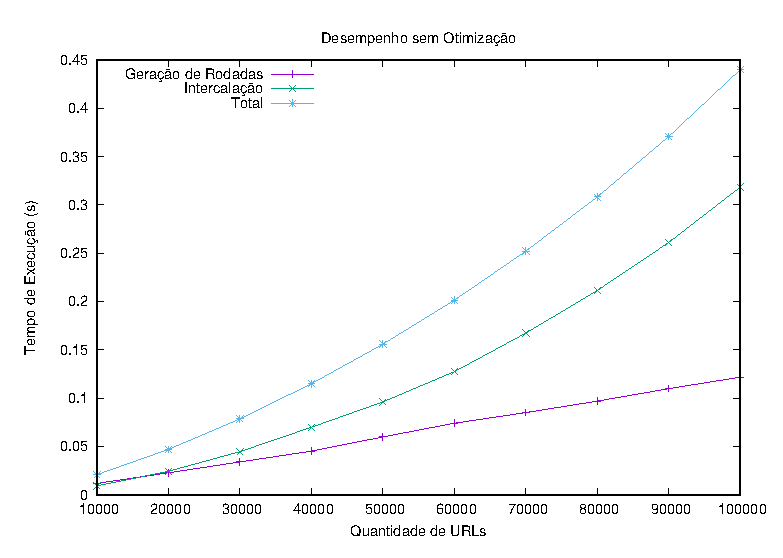
\includegraphics[width=11cm]{not-opt.eps}
	\centering
\end{figure}

\begin{figure}[H]
	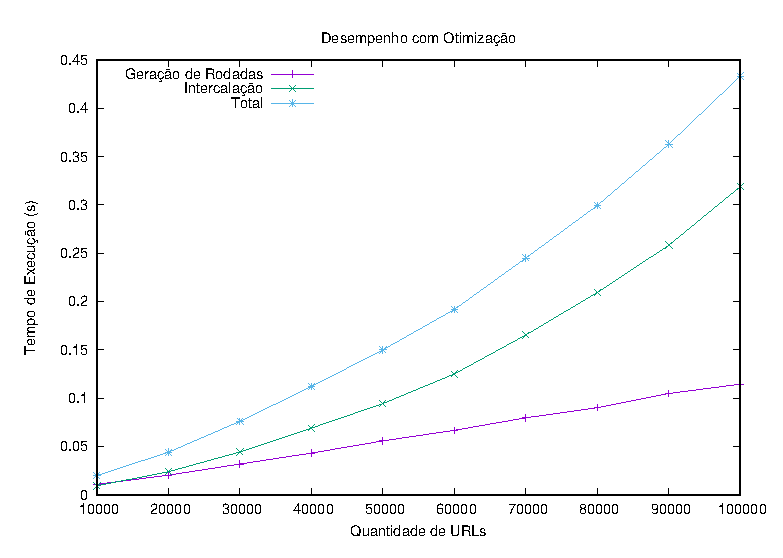
\includegraphics[width=11cm]{opt.eps}
	\centering
\end{figure}

\begin{figure}[H]
	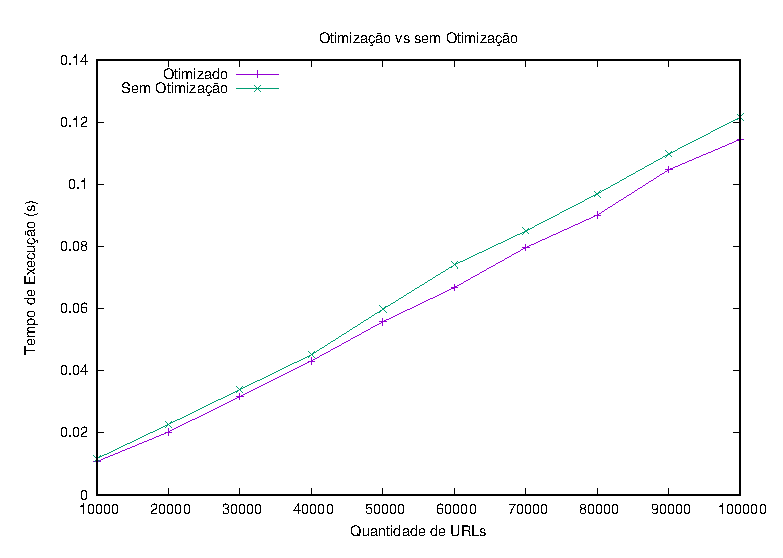
\includegraphics[width=11cm]{qs.eps}
	\centering
\end{figure}

Apesar de a otimização ter se provado consistentemente mais eficiente do que a versão \textit{default}, em muitos casos a melhoria foi negligenciável, distante do \textit{boost} de 40\% esperado. Dos testes que não entraram nessa documentação, às vezes a versão otimizada era até \textit{mais lenta} que a \textit{default} (embora seja possível que essas sejam anomalias). No entanto, dado o perfil linear de ambas as curvas, é possível extrapolar que o uso \textit{InsertionSort} para sub arranjos pequenos trouxe uma melhoria de 5\% na performance.

A ordenação usando o \textit{QuickSort} no pior caso é \( \Theta(n^2) \), mas na prática, esse não é o comportamento esperado, tendendo ao caso médio de \( \Theta(n \log n) \) (como visto em aula). Além da ordenação, nessa etapa também é realizada a leitura e a escrita das rodadas. Na seção 3 foi feita a análise da função \code{sortFitas()} (método que emprega esses 3 procedimentos), de \( \Theta(K \log n) \) (em que \( K \) é o número de linhas do arquivo e \( n \) é o número de páginas por fita, que aqui é constante e igual a 1000). Desse modo, a previsão é de que essa etapa teria caráter linear e de fato foi o que se observou nos resultados. De fato, como esse era o resultado esperado, houve certo viés para escolher baterias de testes que sustentavam essa hipótese, então essa conclusão não é livre de vieses. É importante salientar que não foi feito um tratamento dos dados de forma rigorosa, usando Teste Q e DPR para excluir possíveis anomalias dentro de uma única bateria de testes.

A segunda etapa, de intercalação possui 3 métodos principais: leitura (\( \Theta(n) \), \( n \) número de fitas), construção (\( \Theta(n \log n) \), \( n \) número de fitas) e a própria intercalação (\( \Theta(K \log n) + \Theta(K - n)n \log n \), \( K \) número de URLs e \( n \) número de rodadas). Essa análise pode ser simplificada considerando o fato de que o número de páginas por fita \( m \) é constante (\( m = 1000 \)) nesta aplicação, e que ele relaciona diretamente o número de rodadas e o total de páginas: \( K = n \cdot 1000 \). Assim se simplifica a análise de complexidade para \( \Theta(n) + \Theta(n \log n) + \Theta(1000n \log n) + \Theta(999n^2 \log n) = \Theta(n^2 \log n) \).

As curvas de intercalção, tanto no caso otimixado quanto no padrão, apresentam um caráter parabolóide. No entanto, isso não necessariamente contradiz a previsão da análise: para um dado \( x \) suficientemente grande, a função \( f(x) = x^2 \log x \) se assemelha a uma parábola, uma vez que \( \log x \ll x \) para valores grandes de \( x \). Partindo dessas considerações, o comportamento do gráfico está relativamente dentro do esperado, com inconsistências não muito absurdas. É claro que, como comentado anteriormente, talvez um tratamento mais cuidadoso dos resultados poderia ser usado para se obter uma relação ainda mais clara entre a previsão e a realidade.

Além disso, também foram feitas análises para um tamanho fixo de entrada, variando-se o número de páginas por rodada. Somente foi considerada a versão otimizada do programa. Foi escolhido, arbitrariamente, o tamanho de 10000 páginas, o mesmo arquivo usado na discussão anterior, e variou-se o tamanho do \textit{número de entidades} de 500 em 500 até 4500 (se esse parâmetro for ainda maior, o programa apresenta falha de segmentação).

O resultado parece inconsistente com a análise do método \code{sortFitas()} que prevê \( \Theta(K \log n) \), em que \( K \) é o número de linhas do arquivo (constante, igual a 10000 nessa aplicação) e \( n \) é o parâmetro que está sendo variado. Tal discrepância deve ser relevada ao se considerar o crescimento logarítimo em \( n \) da função: \( \log_2 500 \approx 8.96 \) enquanto que \( \log_2 4500 \approx 12.1 \). Ou seja, é esperado que haja apenas uma pequena diferença nessa etapa, para estes parâmetros.

Para a outra etapa, pode-se considerar a seguinte simplificação: \( n \ll m \Rightarrow m - n \approx m \), de modo que ela passa a ser \( \Theta(mn \log n) \). Como o número rodadas vai diminuindo conforme se aumenta o número de páginas por rodada, obtém-se uma explicação para o perfil do gráfico. De fato, é possível ver que os maiores saltos observados ocorreram justamente quando o aumento de páginas por rodada diminuiu o total de rodadas. No mais, vale ressaltar que o \textit{gnuplot}, por algum motivo, não começou o eixo \( y \) em 0, o que dá a impressão de que os resultados obtidos para tamanhos grandes são muito melhores do que realmente são, quando, na verdade, a proporção entre o pior teste e o melhor teste foi aproximadamente 2.

\begin{figure}[H]
	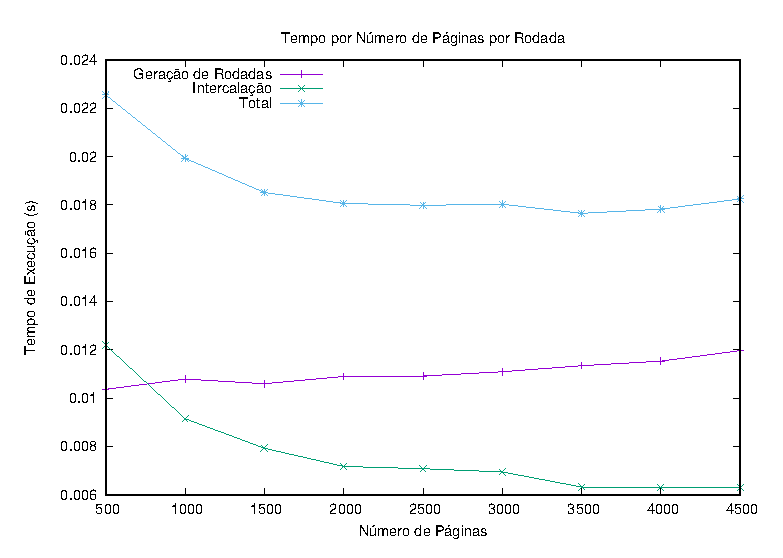
\includegraphics[width=11cm]{rounds.eps}
	\centering
\end{figure}

\subsection{Eficiência de Acesso à Memória}

Nesta subseção são apresentados alguns experimentos que avaliam a eficiência de acesso à memória do programa: padrão de acesso e localidade de referência (distância de pilha). Para realizar essas análises, foi criado um arquivo de 500 linhas usando o \code{geracarga} do professor Wagner Meira Júnior. De fato, os parâmetros para o gerador de carga foram: \code{-o 500\_linhas.txt -u 500 -p 5 -q 1 -r 500 -s 50}. O programa principal foi executado passando 50 como número de ``èntidades'' por fita.

Devido a algumas complicações com o programa para gerar os gráficos, as análises foram fracionadas em diversas partes, explicadas no decorrer do texto. Além disso, essa análise considera exclusivamente as operações relevantes em questão -- no caso da ordenação por exemplo, comparações e trocas.

\subsubsection{Padrão de Acesso}

\begin{figure}[H]
	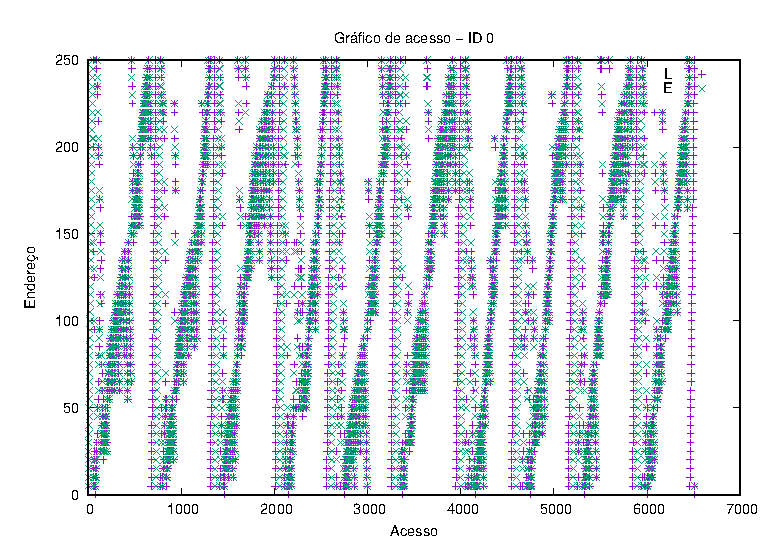
\includegraphics[width=11cm]{1a-fase-acesso-0.eps}
	\centering
\end{figure}

Esse gráfico, que mais se assemelha às imagens do filme Matrix, corresponde à primeira etapa do programa, de gerar as fitas. A princípio, ele pode parecer bem confuso, mas é sim possível extrair informações a partir dele: perceba que o gráfico está fracionado em diversas listras. Cada espaço entre as listas corresponde a uma fita sendo gerada. Como o parâmetro passado foi 50 e o total de linhas no arquivo era 500, as 10 faixas vão de encontro ao que é esperado.

Aqui, no entanto, vale uma consideração: tanto o pivô do \textit{QuickSort} como a variável auxiliar do \textit{InsertionSort} foram desconsideradas pois seus endereços extrapolavam a memória esperada pelo \code{analisamem}, programa que o prof. Wagner disponibilizou para gerar os gráficos a partir dos registros. Foi gerada uma rodada justamente com essas variáveis que ficaram de fora, mas ela não se provou muito interessante, a nível de ser analisada e ter o gráfico incluso nessa documentação. A seguir, é discutida a intercalação.

\begin{figure}[H]
	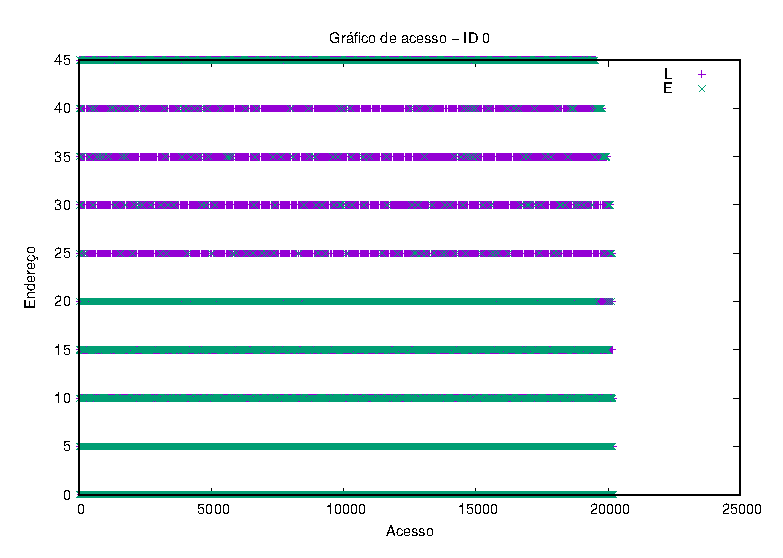
\includegraphics[width=11cm]{2a-fase-acesso-0.eps}
	\centering
\end{figure}

A mesma ressalva da primeira etapa também é aplicada aqui: variáveis de funções internas não foram consideradas ao se gerar o gráfico a cima. Talvez a magnitude de 500 linhas do arquivo seja um impedimento na análise, uma vez que entre 20000 acessos não é possível ver nada de perto. No mais, não foi encontrada nenhuma explicação convincente para os ``saltos'' de 5 em 5 que se pode observar entre os endereços. A grande quantidade de acessos é resultado da constante reconstrução do \textit{heap}, especialmente a função \code{remake()}. A inspeção particular das variáveis deixadas de fora mais uma vez se provou infrutífera.

\subsubsection{Localidade de Referência}

Essa análise, como a anterior, está dividida por etapas (ou seja, execuções diferentes). Ao todo, a DP para os parâmetros supracitados foi de 189443. A seguir são apresentados os histogramas.

\begin{figure}[H]
	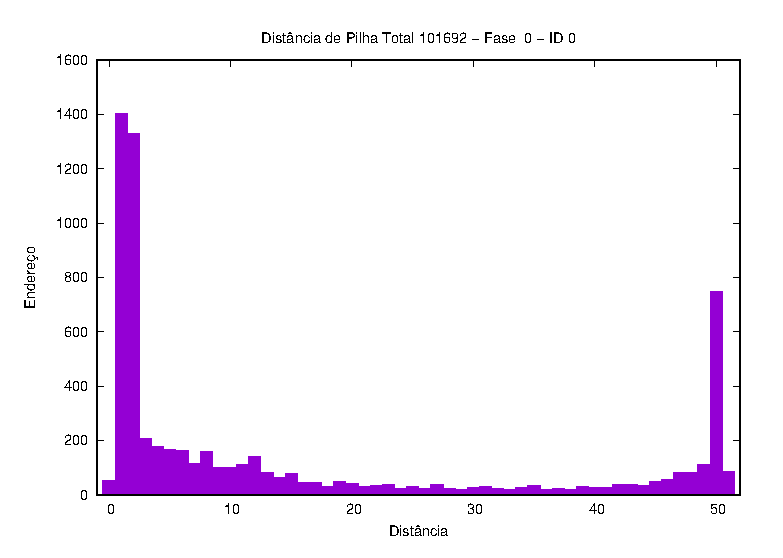
\includegraphics[width=11cm]{1a-fase-hist-0-0.eps}
	\centering
\end{figure}

Na etapa de geração de rodadas, o acesso à pilha é relativamente eficiente: há muitos acessos próximos, embora uma quantia considerável ainda seja alta.

\begin{figure}[H]
	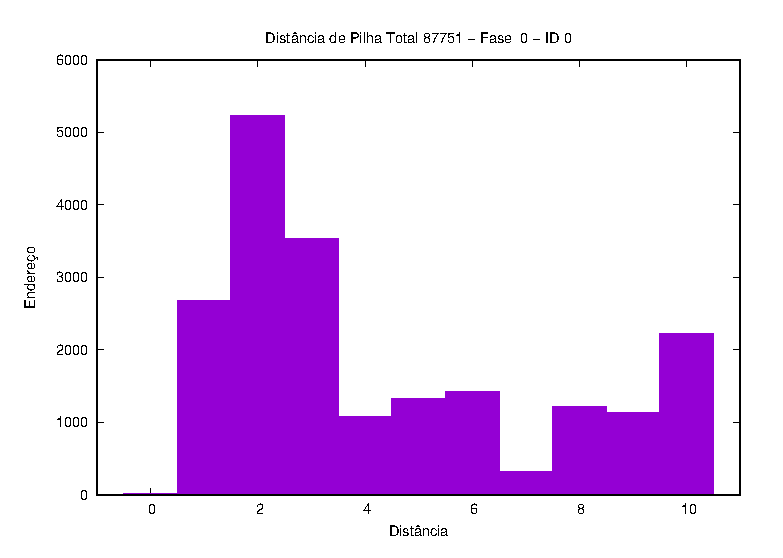
\includegraphics[width=11cm]{2a-fase-hist-0-0.eps}
	\centering
\end{figure}

Na etapa de intercalação também não se pode dizer que a localidade é ruim: a distância nunca é maior que 10, e os valores 1, 2 e 3 são os mais comuns.

\section{Conclusões}

Neste trabalho foi implementado um ordenador de pares \textit{string} e número de um arquivo. Tal par, pode ser considerado uma URL e a sua quantidade de acessos. Foi usado o algoritmo \textit{QuickSort} para realizar a ordenação, e um \textit{heap} para intercalar as fitas.

\subsection{Aprendizado Pessoal}

Em termos de implementação, acredito que foi o TP mais simples dentre os 3 que já fiz. Com \textit{grande} ajuda das aulas, fiz um esboço (em código) do programa em menos de 24 horas, ainda nas férias. O que eu não contava com foi um certo \textit{bug} na intercalação que me fez investir um dia inteiro na busca por uma solução -- eu não estava reconstruindo o \textit{heap} após as inserções, somente o refazendo para uma dada posição, e demorei para notar esse \textit{bug}, tanto é que já tinha feito as análises de performance quando o percebi, e precisei fazê-las novamente. Como no TP1, acho que eu poderia ter elaborado melhor o planejamento de projeto: usar \textit{templates} e classes abstratas.

Mais uma vez estou incerto com as análises de complexidade, até porque não saiu a nota do TP1 ainda, então não sei se venho acertando. Dessa vez consegui fazer as análises de eficiência de acesso à memória, mas acho que ficaram bem medíocres (não sabia exatamente o que comentar em algumas instâncias). Ficam aqui meus agradecimentos ao prof. Wagner Meira Júnior e ao colega Gabriel Teixeira Carvalho na depuração dos erros de segmentação do \code{analisamem}.

Novamente usei um pouco de \textit{shell} para automatizar algumas tarefas da análise de desempenho computacional. Tentei escrever alguns testes de unidade mas acabei desistindo, por mais que dessa vez tivesse o tempo necessário.

\section{Bibliografia}

\begin{enumerate}

	\item PRATES, Raquel. \textbf{Quicksort - Parte1 - Apresentação do método e código}. [S. l.], 19 set. 2020. Disponível em: \url{https://www.youtube.com/watch?v=_5W3jED_9Nc}. Acesso em 10 jan 2022.

	\item PRATES, Raquel. \textbf{Heapsort - Parte1 - O que é um Heap?}. [S. l.], 24 ago. 2020. Disponível em: \url{https://www.youtube.com/watch?v=NVRdSVK8__4}. Acesso em 6 dec 2021.

\end{enumerate}


\newpage
\section*{Instruções}

\subsection*{Compilação}

Você pode compilar o programa da seguinte maneira:

\begin{enumerate}
	\item Utilize o comando \code{cd} para mudar de diretório para a localização da raiz do projeto;
	\item Utilize o comando \code{make}.
\end{enumerate}

\subsection*{Execução}

Você pode rodar o programa da seguinte maneira:

\begin{enumerate}
	\item Utilize o comando \code{cd} para mudar de diretório para a localização da raiz do projeto;
	\item Insira o comando \code{./bin/binary <arquivo-entrada> <arquivo-saída> <número-de-entidades-por-rodada>}. Todos os parâmetros são obrigatórios.
\end{enumerate}

\end{document}
